\documentclass{article}
\usepackage{amssymb} 
\usepackage{amsmath, amsthm}
\usepackage{dsfont}
\usepackage{graphicx}
\usepackage{tikz}



\newtheorem{theorem}{Teorema}[section] 
\newtheorem{proposition}[theorem]{Proposizione} 
\newtheorem{corollary}[theorem]{Corollario}  
\newtheorem{lemma}[theorem]{Lemma}
\theoremstyle{definition}
\newtheorem{esercizio}{Esercizio}
\theoremstyle{definition}
\newtheorem{soluzione}{Soluzione}
\theoremstyle{definition}
\newtheorem{definition}[theorem]{Definizione}
\newtheorem{example}[theorem]{Esempio}

\theoremstyle{remark}
\newtheorem{remark}[theorem]{Osservazione}

\begin{document}
\tableofcontents
\newpage
\section{Algebre e Algebre induttive}
\subsection{Introduzione e definizione}
\begin{definition}[Assiomi di Peano]
    \leavevmode\newline
    \begin{enumerate}
        \renewcommand{\labelenumi}{\Roman{enumi}.}
        \item $\varnothing  \in \mathbb{N}$
        \item  se $n\in\mathbb{N}\implies \sigma(n)\in\mathbb{N}$
        \item $\not\exists n\quad t.c.\quad \sigma(n)= \varnothing$
        \item $\forall m,n \quad \sigma(m)=\sigma(n)\implies n = m$
        \item $\forall S\subseteq \mathbb{N}$ (se $\varnothing \in S$ e $n\in S \implies \sigma(n)\in S)\implies S=\mathbb{N}$
    \end{enumerate}
\end{definition}
Il quinto assioma è equivalente all'induzione, ovvero: sia $P$ una proprietà su $\mathbb{N}$, se $P(0)$ è vera  e si assume sia vera per $n$, quindi
$P(n)$ è vera, se si dimostra che $P(n+1)$ è vero, allora $P$ è vera per ogni $n$. Attraverso questi assiomi abbiamo costruito la "struttura" dei numeri naturali, che non sono altro
che un caso particolare di algebra.
La definizione di peano quindi è un modo per definire un'\textbf{algebra induttiva}. Le algebre sono degli insiemi dotati di operazioni
definite sugli elementi dell'insieme stesso, nel caso delle algebre eterogenee vengono coinvolti anche parametri esterni. Le operazioni definite in questi insiemi
hanno il codominio nell'insieme stesso, consideriamo ad esempio la seguente algebra:

\begin{example}
    Sia $A$ l'insieme dotato di un operazione $\gamma$ definita come segue:
    $$\gamma:  A\times K\to A $$
    dove $K$ è una collezione di elementi diversa da $A$. Anche l'operazione $\eta: K\to A$  che non prende elementi da $A$ può essere un'operazione valida.
\end{example}
\begin{definition}
    Un insieme $S$ si dice chiuso rispetto ad un'operazione $\gamma$ se:
    \begin{enumerate}
        \item $a\in S\implies\gamma(a)\in S$
        \item $a_1,a_2,\dots,a_k\in S\implies \gamma(a_1,a_2,\dots a_k)\in S$
        \item Preso $m\in M$ e $a_1,a_2\in S\implies \gamma(m,a_1,a_2)\in S$
    \end{enumerate}
    (nel (3) $m$ può essere un qualunque elemento di $M$ )
\end{definition}
\begin{definition}
    Un'algebra $(A,\gamma)$, dove $\gamma$ rappresenta una famiglia di operazioni $\{\gamma_i\}$, si dice induttiva quando:
    \begin{enumerate}
        \item Tutte le $\gamma_i$ sono iniettive.
        \item Le $\gamma_i$ hanno immagini disgiunte.
        \item $\forall S\subseteq A$ se $S$ è chiuso rispetto a tutte le  $\gamma_i$ allora $S=A$.
    \end{enumerate}
    L'insieme $A$ è chiamato \textit{insieme sottostante} all'algebra e rappresenta il codominio di ogni operazione $\gamma_i\in \gamma$.
\end{definition}
Quindi $\mathbb{N}$ è solo un caso particolare di algebra induttiva definita su gli interi positivi, dotata dell'operazione $\sigma$ e dell'operazione $\varnothing$.
Quest'ultima merità un piccolo approfondimento, infatti il terzo assioma di Peano impone che $\varnothing$ non sia immagine di alcun $\sigma(n)$, abbiamo quindi bisogno di definire un'operazione speciale
che mappa nello zero:

$$\varnothing: \mathds{1}\to\mathbb{N} $$
Dove $\mathds{1}$ denota l'insieme banale (o $\mathbb{N}^0$ ovvero un insieme composto da un solo elemento). La definizione di algebra induttiva ci serve per definire una collezione di oggetti in cui si esclude tutto ciò che non è
possibile costruire a partire dalle operazioni definite.
\begin{example}[Algebra di liste]
    Definiamo $L$ l'insieme delle liste ordinare di interi e una famiglia di operazioni $\gamma_L$ formata da due operazioni, $cons$, $empty$, diciamo che $(L,\gamma_L)$ è un'algebra induttiva. Definiamo $cons$ come l'operazione che dato un naturale e una lista, aggiunge quel numero in coda alla lista:
    $$cons(n,(n_1,\dots,n_q)) = (n,n_1,\dots,n_q)$$
    $empty$ invece è l'operazione con dominio in $\mathds{1}$ che mappa nella lista vuota $()$. Quindi $cons$ e $empty$ rispettano gli assiomi di algebra induttiva, in particolare: le immagini sono disgiunte, le operazioni sono iniettive e non esistono sotto-algebre chiuse per $cons$ e $empty$.
    Grazie alla struttura induttiva appena costruita possiamo  definire l'operazione $append$, che prende due liste e le unisce. Ecco un esempio di definizione ricorsiva:

    $$append((),l) = l$$
    $$append(cons(n,l),l') = cons(n,append(l,l'))\qquad\text{con $n\in\mathbb{N}$ e $l,l'\in L$}$$


\end{example}
\begin{example}(Booleani) sia $\mathbb{B} = \{True,False\}$ e siano $t,f$ due operazioni:
    $$ t:\mathds{1}\to\mathbb{B}$$
    $$ f:\mathds{1}\to\mathbb{B}$$
    Quindi $t(\mathds{1}) = True$ e $f(\mathds{1}) = False$, da questa definizione segue che  $(\mathbb{B},\{f,t\})$ è un algebra induttiva.
\end{example}
\begin{theorem}
    Un algebra induttiva è finita se e solo se  i costruttori hanno solo parametri esterni.
\end{theorem}
Un esempio banale  è $\mathbb{B}$ $( 1.8)$.
\subsection{Lemma di Lambek}
\subsubsection{Precisazione sulla notazione}
La segnatura algebrica delle operazioni di un'algebra è rappresentata da un'isieme $I$, di nomi di funzione e per ogni $i\in I$ corrisponde un $\alpha_i\ge 0$, che indica il numero di
parametri che l'operazione prende dall' insieme sottostante all' algebra, e un vettore $\mathbf{K_i}=(K_{i1},\dots,K_{iq})$, contente i domini da cui vengono presi i paramentri esterni per l'operazione,
quindi la dimensione del vettore  rappresenta il numero dei parametri esterni.
Due segnature di due algebre sono equivalenti se è possibile ottenere l'una dall'altra semplicemente scambiando gli insiemi sottostanti all'algebra nei singoli costruttori.
\begin{example}
    Consideriamo $(A,f_A)$ e $(B,f_B)$, con $f_A:A\times K \to A$ e \\$f_B:B\times K \to B$, le due algebre hanno la stessa segnatura perché è possibile ottenere $f_A$
        semplicemente sostituendo in $f_B$ $B$ con $A$. Quindi l'equivalenza di segnature è semplicemente un'equivalenza nella "forma" di ogni costruttore dell'algebra.
\end{example}
\begin{definition}  $h:(A,\gamma_A)\to(B,\gamma_B)$ è un omomorfismo di algebre se per ogni $ i\in I$
    $$h(\gamma_{A_i}(a_1,\dots a_{\alpha_i},k_1,\dots,k_{\beta_i})) = \gamma_{B_i}(h(a_1),\dots,h(a_{\alpha_i}),k_1,\dots, k_{\beta_i}). $$
    Un omomorfismo bigettivo è chiamato \textit{isomorfismo}.
\end{definition}
\begin{theorem}
    Siano $(A,\gamma_A)$ un'algebra induttiva e $(B,\gamma_B)$ un'algebra (non necessariamente induttiva), con operazioni con la
    stessa segnatura, allora esiste un unico omomorfismo  $h$:
    $$h:(A,\gamma_A)\to(B,\gamma_B)$$
\end{theorem}
\begin{example}
    Consideriamo l'algebra induttiva dei naturali e $(\mathbb{B},true,not)$, dove $not(true) = false$ e $not(false) = true$. Per il teorema $(1.10)$ esiste un unico omomorfismo di algebre $h:\mathbb{N}\to\mathbb{B}$ definito
    come :
    $$h(\varnothing) = True$$
    $$h(\sigma(n)) = not(h(n))$$
\end{example}
\begin{lemma}[Lambek] Due algebre induttive con stessa segnatura sono isomorfe.
\end{lemma}
\begin{proof}[Dimostrazione]

    Siano $A$ e $B$ due algebre induttive, per $\mathbf{(1.11)}$ esiste un unico omomorfismo $h:A\to B$ e viceversa $h':B\to A$.
    $$A\xrightarrow{h} B\xrightarrow{h'} A$$
    Consiederiamo ora $h'\circ h: A\to A$, ovviamente la composizione di due omomorfismi è anch'esso un omomorfismo, per esempio la funzione identità $Id: A\to A$ è un omomorfismo
    da $A$ in $A$. Ricordiamo che dal precedente teorema sappiamo che tale omomorfismo è unico, segue che $h'\circ h = Id$ e quindi $h' = h^{-1}$.
\end{proof}

Affinchè sia presente un isomorfismo è necessaria una bigezione tra gli insiemi sottostanti all'algebra, ma quest'ultima non è sufficiente a garantire l'uguaglianza nella struttura, infatti
è necessario che anche le segnature siano le stesse.
\begin{example} Prendiamo il caso di due insiemi di interi positivi $\mathbb{N}$ e $\mathbb{N}_*:=\{0,1,\dots,*\}$, esiste certamente una mappa biettiva tra i due insiemi, ma non è possibile stabilire un isomorfismo tra le due algebre, in quanto la segnatura delle rispettive
    famiglie di operazioni sarà diversa.
\end{example}
\subsection{Algebra induttiva di alberi binari}
\begin{theorem}
    Ogni albero binario con $n$ foglie ha $2n-1$ nodi.
\end{theorem}

Per dimosteare questo teorema possiamo utilizzare l'induzione completa, ma ai fini del nostro studio, risulta più istruttivo utilizzare l'\textit{induzione strutturale} su un'algebra induttiva di alberi binari.
Sia $B_{tree}$ l'insieme di tutti gli alberi binari finiti. Dotiamo $B_{tree}$ di due costruttori:
\begin{itemize}
    \item [-] $root : \mathds{1}\to B_{tree}$, un costruttore di base che mappa nell'albero binario formato da un solo nodo.
    \item [-] $branch: B_{tree}\times B_{tree} \to B_{tree}$, un costruttore che unisce due alberi binari, aggiungendo una radice e attaccando i due alberi alla radice, uno come sottoalbero destro e uno come sotto albero sinistro.
\end{itemize}
Le due operazioni rispettano gli assiomi di algebra
induttiva, quindi \\$(B_{tree},root,branch)$ è un'algebra induttiva.
    Possiamo ora applicare l'induzione sull'algebra di alberi binari, modificando l'induzione sui naturali:
    $$ \frac{P(0)\quad P(n)\implies P(\sigma(n))}{\forall n\quad P(n)}\to \frac{P(root)\quad P(t_1),P(t_2)\implies P(branch(t_1,t_2))}{\forall t \quad P(t)}$$

    \begin{proof}[\textbf{Dimostrazione (1.14)}]Il caso base è banale infatti $|root| = 2(1)-1 = 1$. Applichiamo il passo induttivo e dimostriamo che, dati
        $t_1$ e $t_2$ due alberi binari con $|t_1| =2n_1-1$, $|t_2| = 2n_2-1$,  allora $|branch(t_1,t_2)| = 2n_1-1 + 2n_2 -1 +1 = 2(n_1+n_2)-1$.
    \end{proof}

    Durante la costruzione dell'algebra abbiamo specificato la presenza  solo di alberi finiti, in quanto un elemento in sé infinito (in questo caso un albero), violerebbe gli assiomi di algebra induttiva. Quindi le collezioni di elementi con operazioni che contengono elementi di questo tipo
    vengono chiamate algebre \textit{co-induttive}.

    \subsection{Esercizi}
    \begin{definition}
        Un costruttore è  ogni $\gamma_i$ appartenente alla famiglia di operazioni di un algebra $(A,\gamma)$. Un costruttore di base non ha parametri presi dall'insieme sottostante all'algebra, ovvero $\alpha_i = 0$.
    \end{definition}
    \begin{esercizio}
        Dimostrare che ogni algebra induttiva non vuota ha almeno un
        costruttore base.
    \end{esercizio}
    \begin{proof}[\textbf{Soluzione}]Sia $(A,\boldsymbol{\gamma})$, con $\boldsymbol{\gamma} = (\gamma_1,\dots, \gamma_k)$, un'algebra induttiva.
        Consideriamo $\varnothing \subsetneq A$, questo è chiaramente chiuso per ogni $\gamma_i$ che non sia di base, quindi se supponiamo
        che non esistano  in $\boldsymbol{\gamma}$ costruttori di base allora $(\varnothing,\boldsymbol{\gamma})$ è un algebra induttiva, andando in
        contrapposizione con il terzo assioma. Segue l'esistenza di almeno un costruttore base.
    \end{proof}
    \begin{esercizio}
        Mostrare che esiste un isomorfismo algebrico tra i naturali e \\$P =\{0,2,4,\dots\}$
            dove, $0_P = 0$ e $\sigma_P(n) = n+2$.
    \end{esercizio}
    \begin{proof}[\textbf{Soluzione}] Per prima cosa verifichiamo che $(P,\varnothing_P,\sigma_P)$ sia un'algebra induttiva:
        \begin{itemize}
            \item [1.] $\sigma_P$ e $\varnothing_P:\mathds{1}\to P$, sono chiaramente inisettive, infatti se $\sigma_P(n) =\sigma_P(m)$ e quindi
                  $n+2 = m+2\implies n=m$.
            \item [2.] Im $\sigma_P \cap $ Im $\varnothing_P = \varnothing$
            \item [3.] Chiaramente se $S\subseteq P$ è chiuso rispetto a $\varnothing_P$ e $\sigma_P$, allora  $S$ deve essere necessariamente $P$.
        \end{itemize}
        Consideriamo la funzione tra le due algebre induttive che hanno segnature equivalenti:
        $$f: \mathbb{N}\to P$$
        $$n\overset{ f }\longmapsto 2n$$
        Chiaramente $f$ è bigettiva ed è anche un omomofismo, infatti
        $$f(\sigma(n)) = \sigma_P(f(n))$$
        $$\varnothing = \varnothing_P$$
        quindi $f$ è un isomofismo.
    \end{proof}
    \begin{esercizio}
        Dimostrare che ogni algebra induttiva non vuota con un
        costruttore non base è necessariamente infinita.
    \end{esercizio}
    \begin{proof}[\textbf{Soluzione}] Sia $b\in A$  l'elemento mappato dal costruttore di base $\beta$ (di cui abbiamo
        verificato l'esistenza nell'esercizio sopra), se $A$ è dotato anche di un costruttore
        non di base $\gamma$, allora $\gamma(b) = a_1$, $\gamma(a_1) = a_2$ e così via senza mai giungere ad una fine.
        Infatti se volessimo provare a chiudere la sequenza, ad esempio proprio con $\gamma(a_n)=b$, otterremmo delle
        immagini di $\gamma$ e $\beta$ non disgiunte contraddicendo gli assiomi di algebra induttiva, segue la non finitezza di $A$.
    \end{proof}
    \begin{esercizio}
        Consideriamo alberi binari con nodi etichettati da numeri
        naturali. Eccone uno:
        \begin{center}


            \tikzset{every picture/.style={line width=0.75pt}} %set default line width to 0.75pt        

            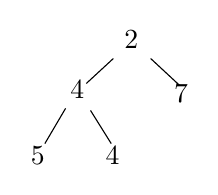
\begin{tikzpicture}[x=0.75pt,y=0.75pt,yscale=-1,xscale=1]
                %uncomment if require: \path (0,300); %set diagram left start at 0, and has height of 300

                %Straight Lines [id:da07036281093773067] 
                \draw    (219,129) -- (209,146) ;
                %Straight Lines [id:da529798846812493] 
                \draw    (241,146) -- (231,130) ;
                %Straight Lines [id:da7883803887618286] 
                \draw    (242,105) -- (229,117) ;
                %Straight Lines [id:da034539223291089605] 
                \draw    (260,105) -- (274,118) ;

                % Text Node
                \draw (246,90.4) node [anchor=north west][inner sep=0.75pt]    {$2$};
                % Text Node
                \draw (220,114.4) node [anchor=north west][inner sep=0.75pt]    {$4$};
                % Text Node
                \draw (201,146.4) node [anchor=north west][inner sep=0.75pt]    {$5$};
                % Text Node
                \draw (270,116.4) node [anchor=north west][inner sep=0.75pt]    {$7$};
                % Text Node
                \draw (237,146.4) node [anchor=north west][inner sep=0.75pt]    {$4$};


            \end{tikzpicture}

        \end{center}
        Definire l’algebra induttiva $BN$-$trees$ di questi alberi.Definire un’algebra di
        uguale segnatura sull’insieme $S$ delle sequenze finite di numeri naturali in modo
        che la funzione $f : BN\text{-}trees\to S$ che associa a ciascun albero la sequenza di
        etichette ottenuta con una visita depth-first sia un omomorfismo. Applicando $f$
        all’albero dell’esempio, ci aspettiamo di ottenere la sequenza ⟨2,4,5,4,7⟩.
        \begin{proof}[\textbf{Soluzione}]
            Definiamo un'estensione delle operazioni create in precedenza per l'algebra di $B_{tree}$:
            $$branch^*: BN\text{-}tree\times BN\text{-}tree\times \mathbb{N}\to BN\text{-}tree,$$
            $$root^*: \mathbb{N}\to BN\text{-}tree.$$
            $branch^*$ prende in input due alberi e un intero che etichetterà la radice; $root^*$ invece prende un
            intero $n$ e crea la radice etichettata con $n$. In modo del tutto analogo definiamo sull'insieme $S$ l'operazione
            di concatenazione di due serie numeriche $s_1, s_2$ di lunghezza dispari che restituisca una serie dispari:
            $$\mathcal{C}:S\times S\times \mathbb{N}\to S$$
            $$\mathcal{C}(s,s',n)\mapsto \langle n,s_1,\dots,s_k,s_1',\dots,s_q'\rangle$$

            $$\Lambda : \mathbb{N}\to S$$
            $$\Lambda(n)\mapsto \langle n\rangle$$
            Come conseguenza del \textit{lemma di Lambek} $(1.12)$ esiste  ed è unico l' omomorfismo $f:B\text{-}tree\to S$.
            Consideriamo la sequenza $s = \langle s_1\dots s_k\rangle$ generata visitando con una $DFS$ l'albero $t\in B\text{-}tree$,
            quindi $f(t) = s$. In particolare $f$ è un omomorfismo di algebre
            \begin{equation}
                f(branch(t_1,t_2,a)) = \mathcal{C}(f(t_1),f(t_2),a)
            \end{equation}
            \begin{equation}
                f(root^*(n)) = \Lambda(n)
            \end{equation}
            La $(1)$ è giustificata dal fatto che la  $depth$-$first$ visita l'albero  da  sinistra a destra, e quindi la sequenza
            risultante avrà inizialmente $a$ (la radice del nuovo albero prodotto da $branch$) $f(t_1)$  ed infine $f(t_2)$.
        \end{proof}
    \end{esercizio}

    \section{Linguaggi di espressioni}
    \subsection{Introduzione}
    \begin{definition}
        Sia $L$ un linguaggio, un insieme di stringhe generate dalla grammatica
        $$M,N ::= 1|2|...|M+N|M*N.$$
    \end{definition}
    \begin{example}
        Ad esempio $3+5$,$3*5$ e $4*5+2$ sono delle espressioni di $L$.
    \end{example}
    Introduciamo la funzione $eval:L\to \mathbb{N}$, per valutare la sintassi delle espressioni:
    $$eval(n) = n$$
    $$eval(M+N) = eval(M) + eval(N)$$
    $$eval(M*N) = eval(M) * eval(N)$$
    Possiamo definire la funzione $eval$ per casi, ma non è stato definito un modo univoco per
    valutare delle espressioni come $\mathbf{"5+4*3"}$, viene svolta prima la $*$ o il $+$ ?\\ Per come è stato costruito il linguaggio $L$ dotato delle operazioni $+$ e $*$ non può essere un'algebra induttiva. Per disambiguare queste espressioni dobbiamo riformulare  il linguaggio in modo da renderlo un algebra induttiva.
    Per iniziare dobbiamo dare una rappresentazione di senso univoco alle espressioni del tipo $\mathbf{"5+4*3"}$, scriviamo più formalemente:
    $$\mathbf{1}:\mathds{1}\to L$$
    $$\mathbf{2}:\mathds{1}\to L$$
    $$\vdots$$
    $$times:L\times L\to L$$
    $$plus :L\times L\to L$$
    Allora $(L,\mathbf{1},\mathbf{2},\dots,times,plus)$ è un'algebra induttiva.
    Quindi l'$eval$ di  $\mathbf{"5+4*3"}$ può essere:
    $$eval(\mathbf{"5+4*3"}) = \left\{ \begin{array}{cl}
            eval(times(plus(\mathbf{5}(\epsilon),\mathbf{4}(\epsilon)),\mathbf{3}(\epsilon))) \\
            eval(plus(\mathbf{5}(\epsilon),times(\mathbf{4}(\epsilon),\mathbf{3}(\epsilon))))
        \end{array}\right.$$
    Pur essendo quella definita sopra la notazione corretta, utilizzarla per le nostre valutazioni risulterebbe
    inutilmente complessa, per questo motivo faremo uso della classica notazione con le parentesi per definire le precedenze.
    Ad esempio $$plus(\mathbf{5}(\epsilon),times(\mathbf{4}(\epsilon),\mathbf{3}(\epsilon))) = 5+(4*3).$$
    \subsection{Linguaggio $\boldsymbol{Exp}$}
    Definiamo il linguaggio $\boldsymbol{Exp}$ costituito da espressioni di somma e $let$:
    $$ M,N ::= k|x|M+N|\text{ let $x = M$ in $N$}$$
    dove $k$ sono le costanti ed appartengono all'insieme dei valori $Val =\{1,2,...\}$; $x$ sono le variabili in $Var=\{x,y,z,\dots\}$ ed $M,N$ in termini di linguaggio in $Exp$.
    \subsubsection{Operatore $\boldsymbol{let}$, variabili \textit{libere e legate}}
    L'operatore $let$ derivante dalla sintassi SML, indicato con $let$ $x=M$ $in$ $N$ e con segnatura:
    $$let : Var \times Exp\times Exp\to Exp$$
    In questo modo definiamo una variabile locale $x$ inizializzata al valore dell' espressione $M$, ed un corpo $N$ che può contenre un riferimento ad $x$. Ad esempio
    $$\text{$let$ $x=4$ $in$ $x+x$}$$
    verrà valutata assegnando alla variabile $x$ il valore $4$, sommando $x+x$ e restituisce $8$.
    Una variabile  è $libera$ in un termine $T$ quando non compare in nessun $N$, sottotermine di $T$, della forma $let$ $x=M$ $in$ $N$.
    Ogni occorrenza di $x$ in $N$ viene detta $legata$ alla dichiarazione di $x$ nel termine $let$ $x=M$ $in$ $N$.
    Definiamo induttivamente la funzione $free:Exp\to \mathcal{P}(Var)$, che restituisce l'insieme delle variabili  che occorrono libere in un'espressione :
    $$free(k) = \varnothing$$
    $$free(x) = \{x\}$$
    $$free(M+N) = free(M)\cup free(N)$$
    $$free(\text{$let$ $x=M$ $in$ $N$}) = free(M) \cup (free(N-\{x\}))$$
    A questo proposito definiamo lo \textit{scoping} di una variabile come l'insieme delle regole che determinano la
    visibilità di una variabile all'interno del programma. Per \textit{scope} di una variabile invece, si intende la porzione di programma in cui la
    variabile può essere riferita.
    \begin{example}
        Consideriamo le due espressioni in $\boldsymbol{Exp}$:
        $$\text{let $x=M$ in let $y=N$ in $L$}  \qquad(I)$$
        $$\text{let $y=$(let $x=M$ in $N$) in $L$}\qquad (II)$$
        Se procediamo alla valutazione di $(I)$ e $(II)$, le due espressioni
        sembrerebbero essere equivalenti, quindi se le intercambiassimo all'interno
        di uno stesso programma, questo dovrebbe produrre lo stesso risultato. Ciò non
        succede nell'espressione qui sotto se valutata:
        $$\text{let $x=1$ in [let $x=M$ in let $y=N$ in $L$]}  \qquad(I')$$
        $$\text{let $x=1$ in [let $y=$(let $x=M$ in $N$) in $L$]}\qquad (II')$$
        In questo caso $(I')$ vale $6$, mentre $(II')$ vale $4$.

    \end{example}
    \subsection{Semantica operazionale di $Exp$}
    Il precedente esempio ci porta a riflettere sull'esistenza di un modo per dimostrare
    l'equivalenza di due programmi. Quest'ultimo è un compito molto più difficile rispetto alla
    dimostrazione della "non equivalenza", la quale solitamente necessità solo di un controesempio.
    Dobbiamo  definire una \textbf{semantica operazionale} per il linguaggio $\boldsymbol{Exp}$ affinché sia possibile assegnare
    un significato alle sue operazioni. Assumeremo, con un'ipotesi semplificata, che il \textbf{significato} di un'espressione sia semplicemente il suo
    valore. Quello che intendiamo creare è un sistema formale con regole di inferenza simile a quello logico, che ci consenta di derivare delle conseguenza a partire da delle premesse iniziali.
    Per definire in modo formale una semantica operazionale è necessario fornire alcune
    nozioni preliminari.
    \begin{definition}
        Una funzione $f$ si dice \textbf{parziale} se può essere definita solo per un sottoinsieme del suo dominio, ed è indicata con la seguente notazione
        $$f: D\rightharpoonup C.$$
        $f$ viene detta \textbf{parziale finita}, se il sottoinsieme del dominio per cui è definita è finito (scritta con $\overset{fin}\rightharpoonup$).

    \end{definition}
    \begin{definition}
        Un \textit{ambiente} è un'associazione tra variabili in $Var$ e valori in $Val$, formalmente definiamo una funzione \textit{parziale finita}
        $$Env:Var\overset{fin}\rightharpoonup Val$$
    \end{definition}
    \begin{definition}
        Siano $E_1$, $E_2$ sono due ambienti, allora la loro composizione $(E_1E_2)$ è quell'ambiente  che se applicato ad una variabile risulta:
        $$(E_1E_2)x =\left\{ \begin{array}{cl}E_2(x) \qquad \text{se definito} \\
                E_1(x) \qquad \text{altrimenti}\end{array} \right.$$
        Quindi per prima cosa si controlla se $x$ è definito nell'ambiente $E_2$, se non definito controlla $E_1$.
    \end{definition}
    \begin{example}$(E_1E_2)(y) = (\{(x,2)(y,3)\}\{(y,4)\})(y) = 4$\end{example}
    \begin{remark}
        Ricordiamo inoltre la forma di una regola logica:
        $$\frac{premessa_1\dots premessa_k}{ conseguenza}\quad(\text{condizione laterale\dots})$$
    \end{remark}
    Risulta necessario sviluppare un insieme di regole che mi permettano, a partire da delle condizioni iniziali, di derivare
    dei sequenti come $E\vdash M \leadsto v$ dove, come specificato precedentemente, $E$ è una funzione parziale $Env$, $M$ è un termine di $Exp$
    e $v$ è un valore in $Val$.
    \begin{definition}La semantica operazionale di $Exp$ è definita come una relazione
        $$\leadsto  \subseteq Env\times Exp\times Val$$
        ovvero una relazione tra $Env$ ed $Exp$ che restituisce un valore in $Val$. Diamo ora una costruzione induttiva
        delle regole della  relazione "$\leadsto$":
        \begin{itemize}
            \item [-] \textit{Regola della costante}: $E\vdash k\leadsto k$
            \item [-] \textit{Regola della variabile}: $E\vdash x \leadsto v$ (se $E(x)= v$)
            \item [-] \textit{Regola del $plus$}: $$\frac{E\vdash M\leadsto v \quad E\vdash N\leadsto u} {E\vdash M+N\leadsto w}\qquad(\text{se $w = u+v$})$$
            \item [-] \textit{Regola del $let$}: $$\frac{E\vdash M\leadsto v \quad E(x,v)\vdash N\leadsto v'}{E\vdash \text{$let$ $x=M$ $in$ $N$}\leadsto v'}$$
                  dove con $E(x,v)$ componiamo l'ambiente $E$ con l'associazione tra $x$ e $v$.
        \end{itemize}
    \end{definition}
    \begin{remark}
        Le premesse in una regola logica non hanno un ordine da seguire, da questo possiamo dedurre
        che la funzione $plus$ sia commutativa. Ovviamente questo non è  vero in ogni linguaggio, ad esempio
        \begin{verbatim}                    x + (x++) != (x++) + x (Java)\end{verbatim}
        Per come è stata costruito il $let$, si potrebbe pensare che provochi una modifica all'ambiente,
        e che quindi sia importante tenere conto dell'ordine con cui viene eseguito, in realtà non è così.
        Infatti la dichiarazione  fatta nel $let$ è limitata all'espressione in $M$ o $N$ che
        sono fatte al suo interno, di conseguenza creeremo solo variabili locali.
    \end{remark}
    \begin{example} La valutazione delle espressioni attraverso la semantica operazionale appena definita viene detta valutazione \textit{eager} ovvero, valuta le espressioni appena le incontra. Diamone la prova utilizzando le regole di derivazione sulla
        seguente espressione (\textit{la valutazione parte dal basso e va verso l'alto}):

        $$\cfrac{\cfrac{\cfrac{(x,1)(y,1)\vdash 2\leadsto 2 \quad (x,1)(y,1)(x,2)\vdash y\leadsto 1}{(x,1)\vdash x \leadsto 1 \quad (x,1)(y,1)\vdash\text{$let$ $x=2$ $in$ $y\leadsto 1$}}}{\varnothing \vdash 1\leadsto 1\quad (x,1)\vdash\text{$let$ $y=x$ $in$ $let$ $x=2$ $in$ $y\leadsto 1$}}}{\varnothing\vdash \text{$let$ $x=1$ $in$ $let$ $y=x$ $in$ $let$ $x=2$ $in$ $y\leadsto 1$}}$$

        Con le regole definite l'espressione è valutata $1$, ma nel caso in cui la valutezione fosse stata \textit{lazy} avremmo ottenuto come risultato $2$,
        questo perché l'espressione viene valutata solo quando dev'essere utilizzata.
    \end{example}
    \subsubsection{Semantica operazionale "\textit{\textbf{lazy}}"}
    Per ottenere una valutazione $lazy$ è necessario modificare la \textit{Regola del let} e la \textit{Regola della variabile}:
    \begin{itemize}
        \item [-] \textit{Regola del let modificata}: $$\cfrac{E(x,M)\vdash N \leadsto v}{E\vdash \text{$let$ $x=M$ $in$ $N\leadsto v$}}$$
              dove $E(x,M)$ indica la composizione dell'ambiente $E$ con l'associazione della variabile $x$ all'espressione non valutata $M$.
        \item [-] \textit{Regola della variabile modificata} $$\cfrac{E\vdash M\leadsto v}{E \vdash x \leadsto v}\quad (\text{se $E(x) = M$} )$$
    \end{itemize}
    In questo modo dobbiamo valutare una certa espressione $M$ solo se è richiesto il suo valore.
    \subsubsection{Semantica \textit{lazy} con \textit{scoping statico}}
    La modifica delle regole oltre a cambiare il tipo
    di valutazione, sta cambiando anche lo $scoping$ del linguaggio. Infatti con la valutazione $eager$ lo scoping era $statico$, ma con l'introduzione delle regole $lazy$ lo scoping è diventato $dinamico$.
    Per ottenere una semantica $lazy$ $statica$ dobbiamo modificare ulteriormente le regole:
    \begin{align*}
         & [let]_{LS} \quad\frac{E(x,M,E)\vdash N \leadsto v}{E\vdash \text{$let$ $x=M$ $in$ $N$}\leadsto v}    \\
         & [var]_{LS} \quad \frac{E'\vdash M \leadsto v}{E\vdash x \leadsto v}\quad (\text{se $E(x) = (M,E')$})
    \end{align*}
    Quello che stiamo facendo è tenere conto dell'ambiente $E$ in cui inizialmente abbiamo l'associazione  $(x,M)$, quindi è necessario
    estendere la funzione $Env$:
    $$Env: Var\overset{fin}{\rightharpoonup} Exp \times Env \quad(I)$$
    La $(I)$ è chiamata \textit{equazione ricorsiva di domini}, la soluzione dell'equazione è ogni insieme $X$ per cui
    $$X : Var\overset{fin}{\rightharpoonup} Exp \times X$$
    in particolare possiamo avere una soluzione con \textit{ambienti alti}, ovvero una serie di ambienti infinitamente annidati; altrimenti avremo degli $ambienti$ $bassi$.
    Risulta chiaro che un ambiente $alto$ ad esempio
    $$E = \{(x,\{(x,\{(x,\{\dots\}\dots)\}$$
    non terminerà mai la valutazione di $x$ nel caso in cui ne avesse bisogno.
    Nel caso dello \textit{scoping statico} tengo conto dell'ambiente in cui ho eseguito una determinata associazione;
    se invece lo \textit{scoping} è $dinamico$ utilizzo l'ambiente attuale per eseguire la valutazione.
    \begin{remark}
        La valutazione $lazy$ non è sempre più efficiente di quella $eager$, infatti ogni volta che avremo bisogno di un valore, se utilizziamo la $laziness$ dobbiamo ricalcolarlo per ogni occorrenza. Ad esempio
        $$\text{$let$ $x = M$ $in$ $x+x+x+x+x$}$$
        se $M$ è un termine complesso, la valutazione $lazy$ è estremamente inefficiente.
    \end{remark}
    \begin{example}
        Valutiamo la seguente espressione con la semantica $lazy$ $statica$:
        $$\cfrac{\cfrac{\cfrac{\cfrac{\cfrac{\varnothing \vdash 3 \leadsto 3}
                        {E \vdash x \leadsto 3}\quad (E(x) = (3,\varnothing))}
                    {E'' = E'(x,5,E')\vdash y \leadsto 3}(E''(y) = (x,E))}
                    {E' = E(y,x,E)\vdash \text{$let$ $x=5$ $in$ $y$}\leadsto 3}}
                {E = (x,3,\varnothing)\vdash \text{$let$ $y= x$ $in$ $let$ $x=5$ $in$ $y$}\leadsto 3}}
            {\varnothing\vdash \text{$let$ $x=3$ $in$ $let$ $y= x$ $in$ $let$ $x=5$ $in$ $y$}\leadsto 3}$$
        La valutazione sarebbe stata la stessa se avessimo utilizzato le regole della sematinca $eager$.
    \end{example}
    \begin{definition}
        Un ambiente $eager$ $E$ si dice $equivalente$ ad un ambiente $lazy$ $statico$ $E'$, se per ogni variabile $x$,  con $E(x)=v$, esistono $M$ ed $E''$ tali che $E'(x) = (M,E'')$ e $E''\vdash M \leadsto v$.
    \end{definition}
    \begin{theorem}Le semantiche $lazy$ $statica$ e $eager$ sono equivalenti se e solo se $E$ ed $E'$ non sono ambienti $alti$.

        $$E\vdash M \leadsto_E v \iff E' \vdash M \leadsto_{LS} v$$
    \end{theorem}
    \section{Linguaggio \textit{Fun}}
    Il linguaggio $Fun$ estende il linguaggio $Exp$ con la nozione di $funzione$, quindi possiamo aggiungere al precedente linguaggio le seguenti clausole:
    $$ \text{$fn$ $x$} \implies M|MN,$$
    quindi
    $$MN ::= k|x|M+N|\text{$let$ $x=M$ $in$ $N|$ $fn$ $x$ }\implies M|MN$$
    Successivamente mostreremo che le clausole definite nel linguaggio $Exp$, ad eccezione delle $variabili$ non sono necessarie in $Fun$. L'operazione $fn$ ha segnatura:
    $$fn: Var\times Fun \to Fun$$
    \begin{remark}
        L'operazione $fn$ prende una sola variabile in input, per costruire "funzioni a più variabili" possiamo comporre più operatori $fn$
        $$\text{$fn$ $x_1 \implies (fn$ $x_2\implies$\dots($fn$ $x_k\implies M$) }$$
        Per comodità la notazione sopra sarà equivalente a $fn$ $x_1\dots x_k\implies M$.
    \end{remark}
    \begin{example}
        $fn$ $xy\Rightarrow x+y$, nella scrittura completa $fn$ $x\Rightarrow fn$ $y\Rightarrow x+y$.
        Utilizzando la clausola $fn$ $x\Rightarrow MN$ stiamo applicando $M$ ad $N$, ad esempio
        $$\text{$(fn$ $xy\rightarrow yx)$$(fn$ $x\Rightarrow x+1)$$(fn$ $x\Rightarrow x)3$}$$
        In questo caso a la prima funzione a partire da sinistra inverte l'ordine di applicazione delle due funzioni che la seguono,
        applicando la funzione identica e poi la funzione successore, successivamente passo $3$ alla funzione successore ottenendo $4$.
    \end{example}
    \subsection{Semantica operazionale}
    Essendo $Fun$ un'estensione del linguaggio  $Exp$ diamo ora un'estensione anche delle regole semantiche. Per iniziare nell'espressione
$\text{$fn$ $x\Rightarrow M$}$  non c'è nulla da calcolare, per questo potremmo dire che
    $$\text{$fn$ $x\Rightarrow M$}\leadsto \text{$fn$ $x\Rightarrow M$}\qquad \qquad(*)$$
    Useremo la notazione della $chiusura$ per esprimere la parte sinistra della relazione  $(*)$, indicata con
    $$[fn]\quad\text{$fn$ $x\Rightarrow M$}\leadsto (x,M)\qquad \qquad (I)$$
    dove $M$ è il $corpo$ della $chiusura$, mentre $x$ è il $parametro$. A seguito di questa
    modifcia è necessario un ulteriore cambiamento nel dominio $Val$ nella relazione $\leadsto$:
    $$Val = Const \cup (Var\times Fun)$$
    dove $Const = \{5,6,\dots\}$.
    Studiamo ora il significato dell' applicazione di $M$ ad $N$ espressa con $MN$. Affinché tale espressione possa essere valutata è necessario
    che $M$ sia una funzione, inoltre in questa prima definizione adotteremo una semantica $eager$ con $scoping$ $dinamico$.
    $$[appl]\quad\frac{E\vdash M \leadsto (x,M') \quad E \vdash N\leadsto v \quad E(x,v)\vdash M'\leadsto v'}{E\vdash MN\leadsto v'}\qquad \qquad (II)$$
    quindi, per valutare $MN$  dobbiamo valutare per prima $M$  all'interno di $E$ e restituire la sua $chiusura$, successivamente "passare"
    alla funzione appena valutata $N$ (creando l'associazione $(x,v)$), infine valutare $M'$, ovvero il corpo della $chiusura$, nell'ambiente $E$ aumentato dell'associazione
    di $v$ ad $x$.
    \begin{remark}
        Bisogna ricordare che $v$ e $v'$ non rappresentano più solo dei valori.
    \end{remark}
    \begin{example}
        Deriviamo con la semantica appena definita la seguente espressione:
        $$\cfrac{\cfrac{\cfrac{E\vdash y\leadsto (z,x+z)\quad E\vdash 7\leadsto 7\quad E(z,7)\vdash x+z \leadsto 10}{(x,3)\vdash \text{$fn$ $z\Rightarrow x+z$}\leadsto (z,x+z)\quad E =(x,3)(y,(z,(x+z)))\vdash \text{$let$ $x=4$ $in$ $y7\leadsto 10$}}}
                {\varnothing\vdash 3\leadsto 3 \quad (x,3)\vdash\text{$let$ $y = (fn$ $z\Rightarrow x$) $in$ $y7\leadsto 10$}}}
            {\varnothing \vdash \text{$let$ $x=3$ $in$ $let$ $y = (fn$ $z\Rightarrow x$) $in$ $y7\leadsto 10$ }}$$
    \end{example}
    Definendo la semantica di $Fun$ con approccio $eager$ abbiamo ottenuto uno scoping $dinamico$, questo perchè  il $corpo$ della $chiusura$ non viene valutato immediatamente (appena viene dichiarata la funzione), in aggiunta
    al fatto che non memorizziamo l'ambiente in cui inizialmente è dichiarata. Per ottenere quindi un \textbf{\textit{eager statico}} è sufficiente modificare la $chiusura$ memorizzando oltre al parametro e al corpo, anche l'ambiente
    del momento in cui incontriamo la funzione.
    Quindi la $(I)$ diventa
    $$E\vdash\text{$fn$ $x\Rightarrow M$}\leadsto(x,M,E)$$
    mentre la regola $(II)$ (\textit{regola di applicazione}) sarà
    $$\frac{E\vdash M \leadsto (x,M',E) \quad E \vdash N\leadsto v \quad E'(x,v)\vdash M'\leadsto v'}{E\vdash MN\leadsto v'}\qquad \qquad (II)$$
    Possiamo convincerci della validità di questa modifica provando a valutare il termine qui sotto, che avrà valore $4$ nel caso di $eager$ $dinamico$, $3$ con quello $statico$:
    $$\varnothing\vdash \text{$let$ $x=3$ $in$ $let$ $y=fn$ $z\Rightarrow x$ $in$ $let$ $x=4$ $in$ $y7$.}$$
    Per ottenere una versione \textbf{\textit{lazy}} di $Fun$ possiamo estendere la versione $lazy$ di $Exp$, modificando anche le regole di $applicazione$ e quella di $fn$.
    \subsection{Il lambda calcolo}
    Avremmo potuto scrivere il linguaggio $Fun$ in termini più semplici eliminando delle clausole che sono derivabili da altre. Ad esempio la clausola
    $$\text{$let$ $x=M$ $in$ $N \equiv$ ($fn$ $x\Rightarrow N)M$  }$$
    intuitivamente sia a sinistra che a destra stiamo applicando $M$ in $N$.
    \begin{proof}[\textbf{Dimostrazione}]
        La regola $[let]$ di $Fun$ può essere derivata dalle regole  $[appl]$ ed $[fn]$. Infatti $[let]$ deriva $let$ $x=M$ $in$ $E\vdash N\leadsto v$ a partire dalle premesse
        $E\vdash M\leadsto v'$  e $E(x,v')\vdash N \leadsto v$. \\Quindi  traducendo il termine $let$ in  $(fn$ $x\Rightarrow N)M$ riusciamo comunque a derivare $v$, a partire dalle stesse premesse  con l'aggiunta della assioma $[fn]$:
        $$\frac{E\vdash \text{$fn$ $x\Rightarrow N\leadsto (x,N,E)$}\quad E\vdash M\leadsto v' \quad E(x,v')\vdash N \leadsto v  }{E\vdash \text{$(fn$ $x\Rightarrow N)M\leadsto v$}}$$
    \end{proof}
    In modo simile possiamo eliminare anche tutti i valori in $Val$ e la somma ($M+N$) ottenendo
    $$M,N ::= x|\text{$fn$ $x\Rightarrow M|MN$}$$
    questo linguaggio più semplice  sarà chiamato $lambda$ $calcolo$ e i suoi termini, $lambda$ $termini$.
    \subsubsection{I numeri di Church}
    Il $lambda$ $calcolo$ appena definito deve essere equivalente al linguaggio $Fun$, quindi deve esistere un modo
    per rappresentare i numeri in $Val$ che abbiamo eliminato, e di conseguenza anche la loro aritmetica.
    Una rappresentazione di questi numeri tramite il $lambda$ $calcolo$ è stata data da $Alonzo$ $Church$. Essendo
    il $\lambda$-calcolo un linguaggio di sole funzioni, per esempio, $tre$ viene definito come :
    $$c_3 = fn\text{ $xy\Rightarrow x(x(xy))$}$$
    in parole \textit{"applico 3 volte x a y"}. In generale un numero $n\in \omega$ può essere scritto

    $$c_n = fn\text{ $xy$}\Rightarrow x^n y$$
    $$c_0 = fn\text{ $xy$}\Rightarrow  y$$

    Definiamo ora la funzione successore per i numeri di Church $\sigma$, che prende in input un numero di Church e ne ritorna il successore:
    $$\sigma(w) \equiv fn\text{ }w\Rightarrow fn\text{ }xy \Rightarrow wx(xy)\equiv x(wxy)$$
    \textit{Spiegazione:} partiamo da un numero di Church $w$, e otteniamo il suo successore applicando $x$ ad $y$ una volta (ovvero ($xy$)),  successivamente applichiamo ad $(xy)$, $w$ volte $x$ ($w$ è la funzione che si applica $w$ volte a qualcosa dato in input).
    Con l'aiuto della funzione successore possiamo definire l'operazione $plus$ per i numeri di Church:
    $$plus\:u\,v = w \sigma v$$
    ovvero passo $\sigma$ a $w$, cioè la funzione che la applica $w$ volte, e applico questa composizione a $v$. In modo simile e con risultato del tutto analogo
    possiamo scriverla come
    $$fn \text{ $wv\Rightarrow$ $fn$ $xy\Rightarrow wx(vxy)$ }$$
    quindi applichiamo la funzione $x$, $v$ volte ad $y$ e passo il risultato a $w$, che applica per altre $w$ volte $x$ ad $y$.
    Continuando la costruzione dell'aritmetica definiamo la moltiplicazione $times$ a partire dal $plus$:
    $$fn\, uv\Rightarrow v(plus\, u)\:c_0$$
    oppure
    $$fn\: uv\Rightarrow fn\: xy\Rightarrow u(vx)y.$$
    \textit{Spiegazione:} applico $u$ alla funzione che applica $v$ volte  $x$ a qualcosa, ovvero $(vx)$, il risultato è la funzione che applica $u$ volte  $(vx)$, ovviamente ad $y$.
\end{document}
